\section{Experimental validation}
\label{sec:exps}

%
% Corpus
%


We experimented our models and inference on several real world, either directed or undirected, networks. Theirs statistics and properties are summarized in table \ref{table:corpus}. The detailed descriptions are available in the online Koblenz network collection\footnote{http://konect.uni-koblenz.de/}.

\begin{table}[h]
\bgroup
\def\arraystretch{1} % 1 is the default, change whatever you need
	
\caption{Datasets networks used to train the models. Type A is for co-authorship, type C is for communication, type H is for hyperlinks, type L is for lexical network and I for interaction network.}

\resizebox{\textwidth}{!}{
\begin{tabular}{lrrrrcrrrr}
%\Xhline{2\arrayrulewidth}
\toprule
 Datasets     &   Nodes &   Edges &   Density & Directed  &    Diameter &   \multicolumn{3}{c}{Weights}  	& type     \\
 \cmidrule(l){7-9}  &   &   	  &   $\times 10^{-3}$		  & 		  &  		   	&  mean & std  & max             \\
%\hline
\midrule
astro-ph      & 16,706  & 121,251   & 0.87  & False & 14 & 1.8  & 3.3  & 306  & A  \\
%cond-mat     & 16,726  & 47,594    & 0.000 & False & 18 & 3.1  & 7.2  & 544  & A  \\
hep-th        & 8,361   & 15,751    & 0.45  & False & 1  & 5.2  & 16   & 1226 & A  \\
%netscience   & 1,589   & 2,742     & 0.002 & False & 2  & 2.2  & 1.9  & 33   & A  \\
moreno\_names & 1,773   & 9,131     & 5.81  & False & 8  & 1.8  & 3.0  & 100  & L  \\
manufacturing & 167     & 5,783     & 208   & True  & 3  & 14.3 & 44.9 & 1458 & C  \\
fb\_uc        & 1,899   & 20,296    & 5.63  & True  & 4  & 2.8  & 4.7  & 98   & C  \\
digg\_reply   & 30,398  & 85,247    & 0.09  & True  & 11 & 2.0  & 0.2  & 26   & C  \\
slashdot      & 51,083  & 130,370   & 0.05  & True  & 11 & 2.1  & 0.3  & 18   & C  \\
enron         & 87,273  & 320,154   & 0.04  & True  & 15 & 3.4  & 12.4 & 3904 & C  \\
wiki-link     & 100,312 & 887,426   & 0.09  & True  & 14 & 1.7  & 3.0  & 185  & H  \\
prosper-loans & 89,269  & 3,330,225 & 0.42  & True  & 2  & 2.0  & 0.2  & 16   & I  \\
%\Xhline{2\arrayrulewidth}
\bottomrule
\end{tabular}
}


\egroup
\label{table:corpus}
\end{table}



%
% Evaluation method (testing set and mesure)
%
To evaluate the performance of the models and to illustrate the advantage of the online inference, we designed a experiments based on different size of training set to test the impact of the amount of data on the inference. For all the dataset, we first built a test set  by extracting randomly 20 percent of the edges of the networks and about the same amount of non-links. The remaining data consitute the "full" training set. Then, we subsampled the full training set in order to obtain "sub" training set containg different propotions of the edges (i.e 1, 5, 10, 20, 30, 50, and 100 percent, the former corresponfing to the full trainig set.). Furthermore, we ensure that all the sub training set are inclusive. We repeated this settings 10 times with different seed, to cross validate our results.

The all our models implemented with the stochastic collapsed variationnal inference, we set the gradient step parameters to $\tau=1024$ and $\kappa=0.5$, the burn-in period to $T_{burnin}=150$ and for the stratidied sampling, we fix the paramter $M=50$. For MMSB we set the hyperparameters $\lambda_0=\lambda_1=0.1$ and for MMSB, WMMSB and WMMSB-bg we set the latent-class hyperparameters to $\alpha_k=\frac{1}{K}$ and the number of latent classes to $K=10$.

% stopping citerion
For the stopping criteria of the inference, we further held-out 10 percent of the remaining training set is held-out during the inference. The log-likelihood is computed at after each minibatche. When the log-likelihood average increase (on the last 20 measures) is less that 0.001, the inference is stopped. The log-likelihood of a  given set of observations $\D_{test}$  is computed as follows:
\begin{equation*}
\log p(\D_{test}) = \sum_{i,j \in \D_{test}} \log p(y_{ij} | \phih_{kk'}) p(k|\thetah_i) p(k'|\thetah_j)
%\log p(\D_{test}) = \sum_{i,j \in \D_{test}} \log p(y_{ij} | \phih_{kk'}) p(k|\thetah_i) p(k'|\thetah_j)
\end{equation*}



\textcolor{white}{ % trick to make it invisible, only in the footpage.
\footnote{\url{http://konect.uni-koblenz.de/networks/ca-AstroPh}. We used the cleaned version available in the  graph-tool framenetwork.}
\footnote{\url{hhttp://konect.uni-koblenz.de/networks/ca-cit-HepTh}. We used the cleaned version available in the  graph-tool framework.}
\footnote{\url{hhttp://konect.uni-koblenz.de/networks/moreno_names}}
\footnote{\url{hhttp://konect.uni-koblenz.de/networks/radoslaw_email}}
\footnote{\url{hhttp://konect.uni-koblenz.de/networks/opsahl-ucsocial}}
\footnote{\url{hhttp://konect.uni-koblenz.de/networks/munmun_digg_reply}}
\footnote{\url{hhttp://konect.uni-koblenz.de/networks/slashdot-threads}}
\footnote{\url{hhttp://konect.uni-koblenz.de/networks/enron}}
\footnote{\url{hhttp://konect.uni-koblenz.de/networks/link-dynamic-simplewiki}}
\footnote{\url{hhttp://konect.uni-koblenz.de/networks/prosper-loans}}
}


\begin{figure}[h]
\centering
	

\begin{subfigure}
     \centering
         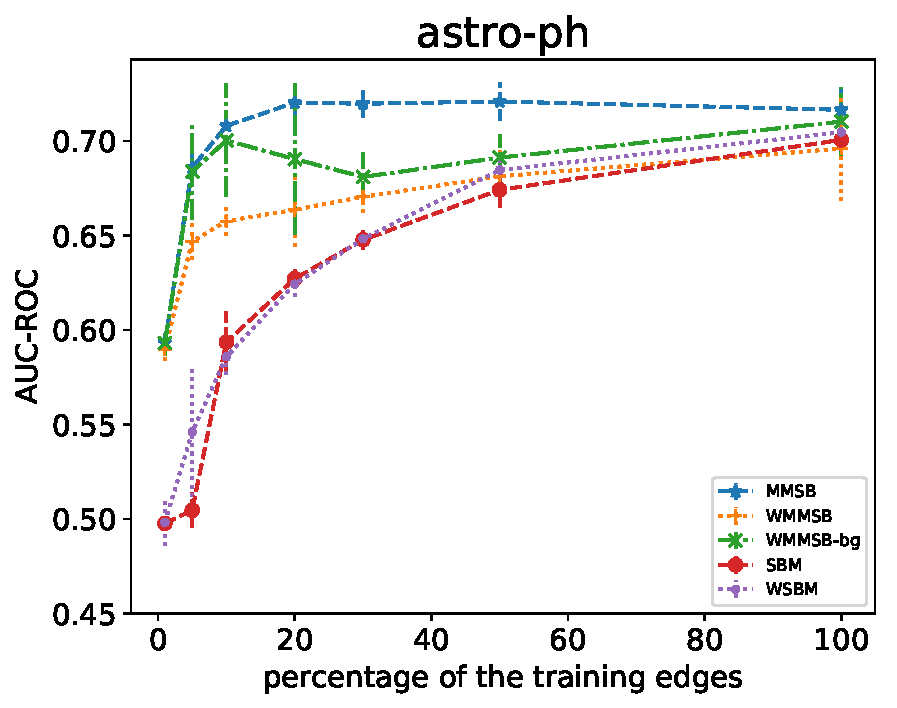
\includegraphics[width=0.32\textwidth]{fig/astro-ph__entropy@_roc_evo}
\end{subfigure}
\begin{subfigure}
         \centering
      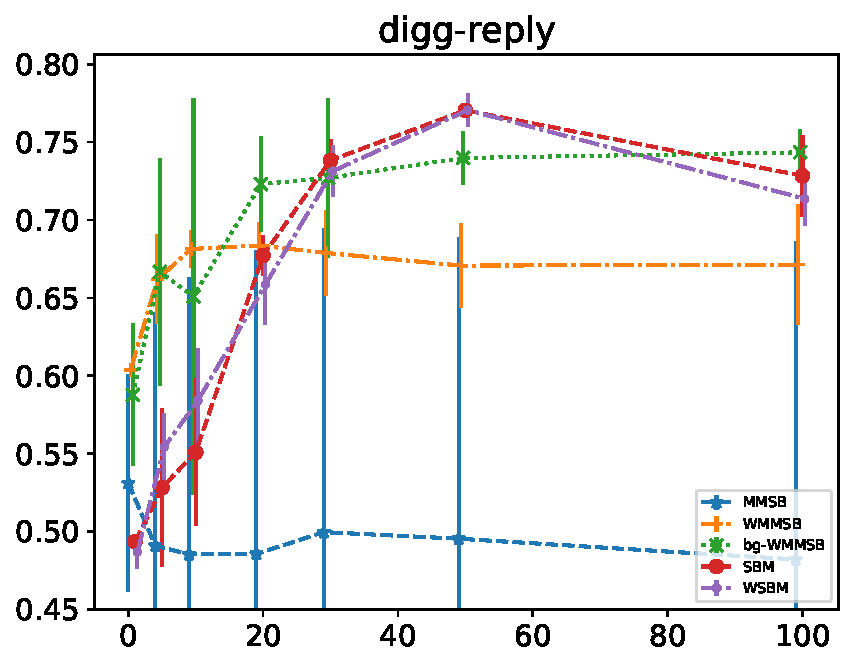
\includegraphics[width=0.32\textwidth]{fig/digg-reply__entropy@_roc_evo}               
\end{subfigure}                                                                          
\begin{subfigure}                                                                        
         \centering                                                                      
      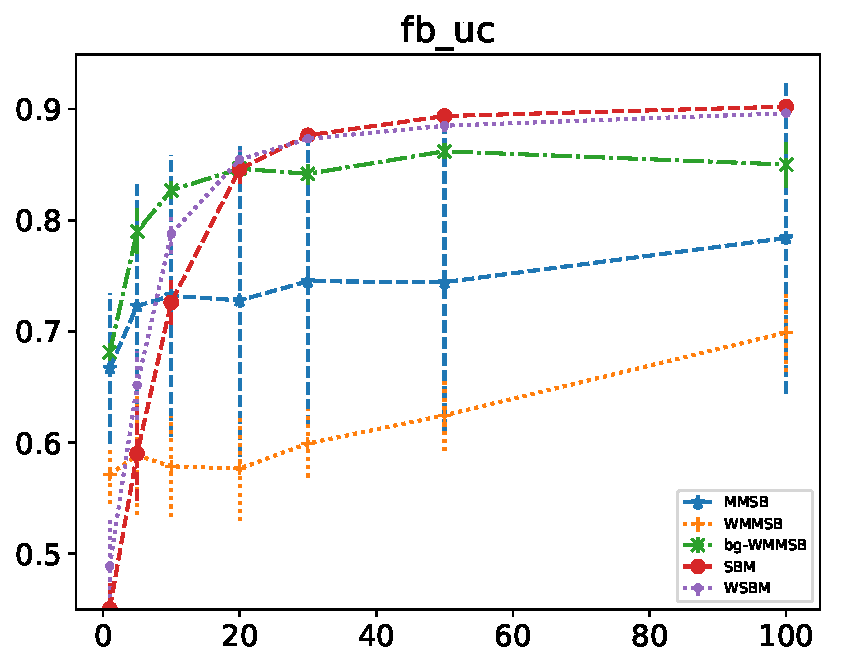
\includegraphics[width=0.32\textwidth]{fig/fb_uc__entropy@_roc_evo}
\end{subfigure}                                                                          
\begin{subfigure}                                                                        
         \centering                                                                      
      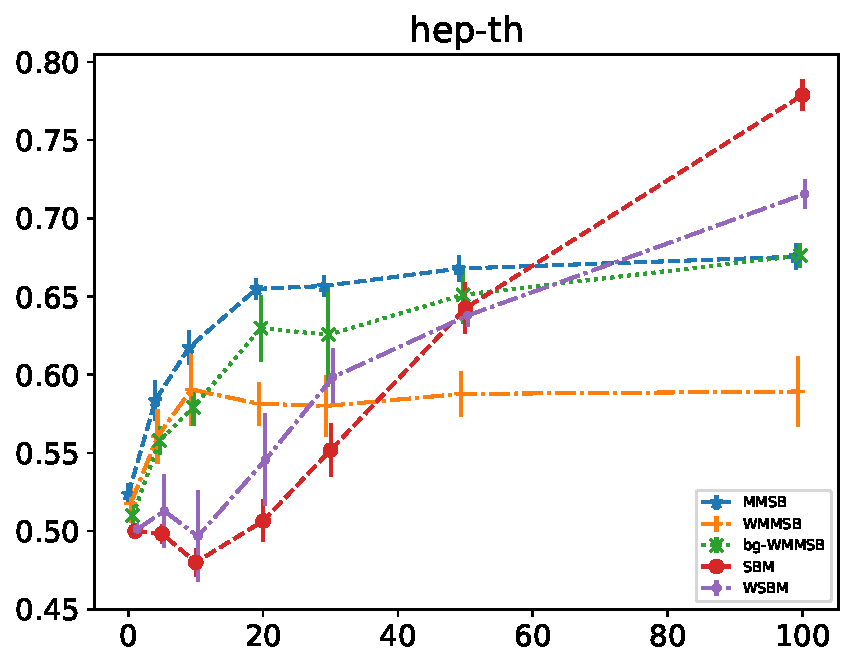
\includegraphics[width=0.32\textwidth]{fig/hep-th__entropy@_roc_evo}
\end{subfigure}                                                                          
\begin{subfigure}                                                                        
     \centering                                                                          
         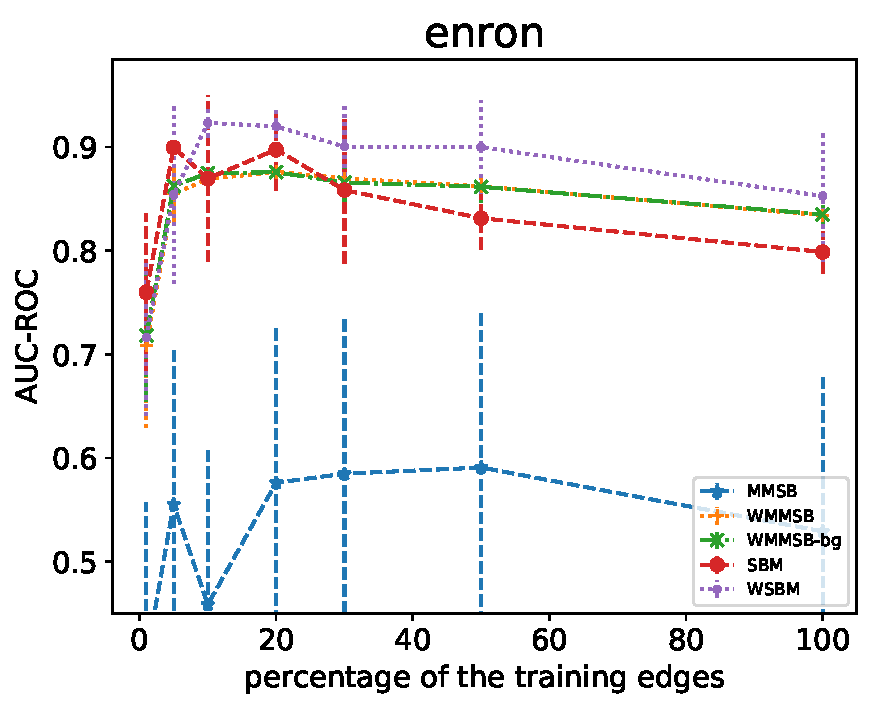
\includegraphics[width=0.32\textwidth]{fig/enron__entropy@_roc_evo}
\end{subfigure}
\begin{subfigure}
         \centering
      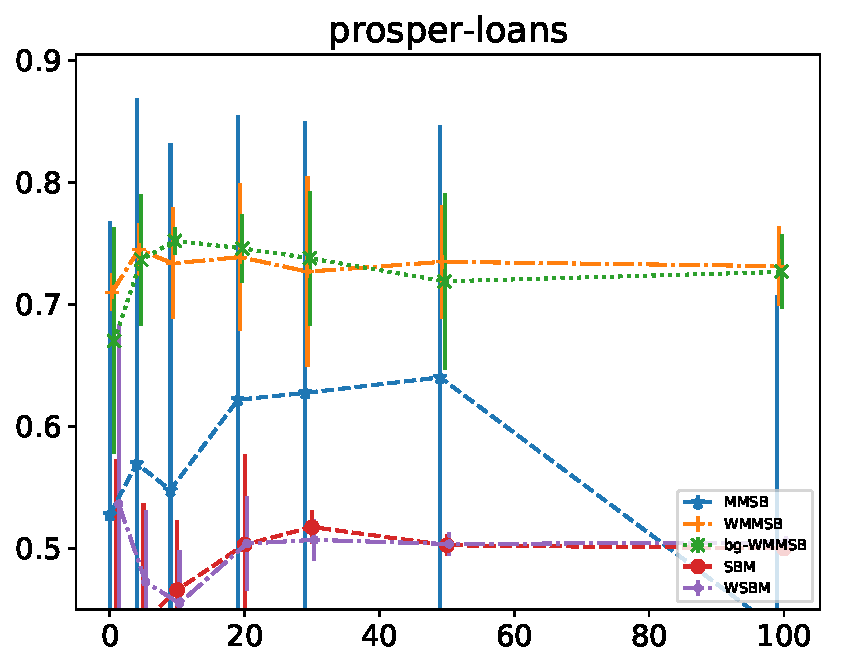
\includegraphics[width=0.32\textwidth]{fig/prosper-loans__entropy@_roc_evo}
\end{subfigure}                                                             
\begin{subfigure}                                                           
         \centering                                                         
      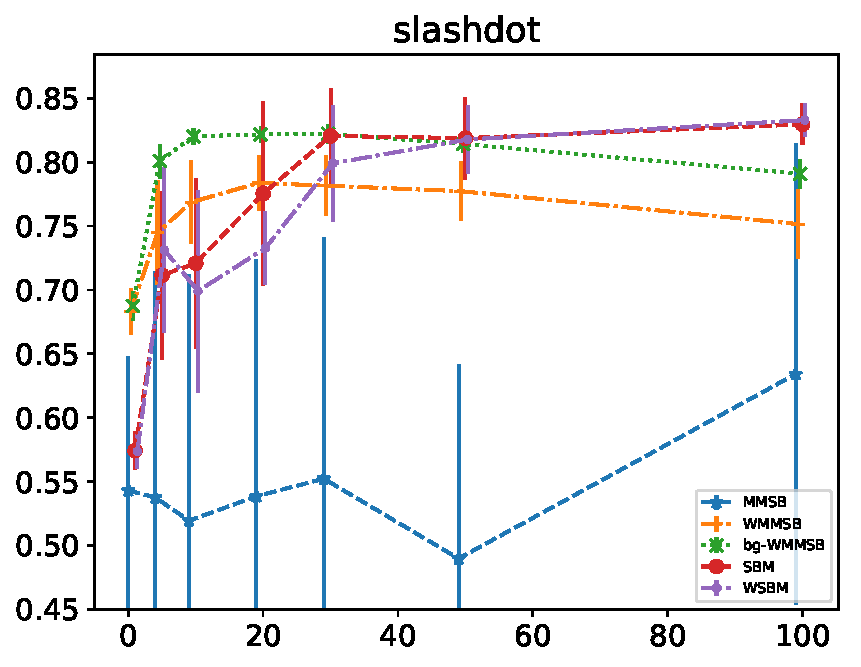
\includegraphics[width=0.32\textwidth]{fig/slashdot__entropy@_roc_evo}
\end{subfigure}                                                             
\begin{subfigure}                                                           
         \centering                                                         
      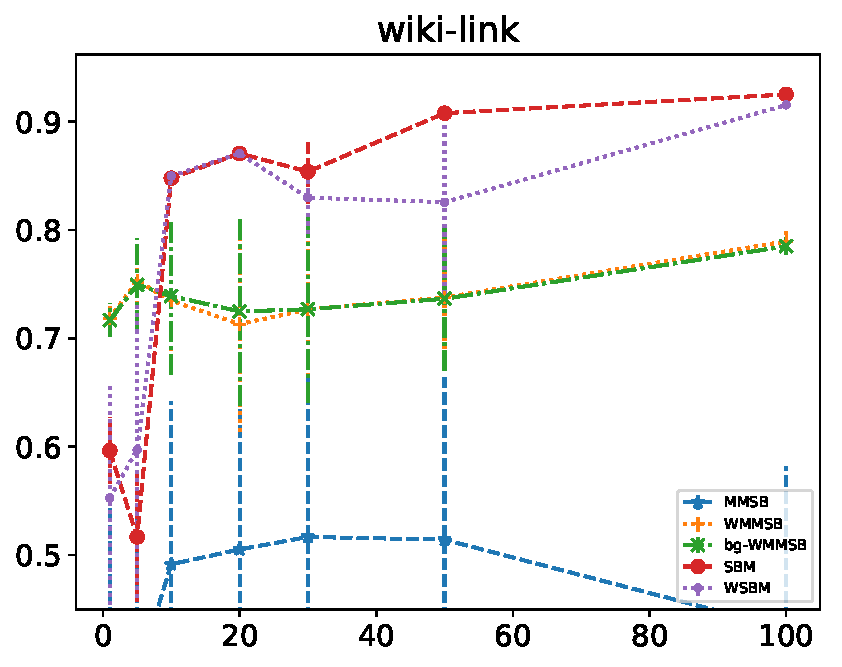
\includegraphics[width=0.32\textwidth]{fig/wiki-link__entropy@_roc_evo}
\end{subfigure}                                                             
\begin{subfigure}                                                           
         \centering                                                         
      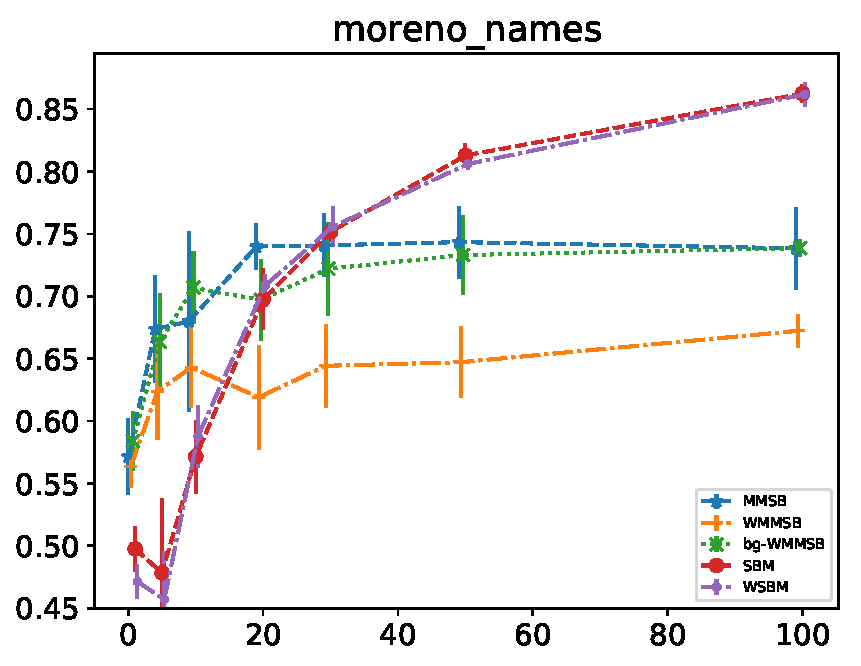
\includegraphics[width=0.32\textwidth]{fig/moreno_names__entropy@_roc_evo}
\end{subfigure}                                                             
\caption{Comparison of models in terms of AUC-ROC scores according to the percentage of edges used to train the models (from 1 to 100\%).}


   \label{fig:roc}
\end{figure}


In order to carachterize to wich extent the models can predict the missing links of the networks, an thus recover its topology. For the weighted models, the probability to observe a links is computed as the probability that at least one edge count is generated by:
\begin{equation*}
p(y_{ij} \geq 1 | \Thetah, \Phih) = 1 - \sum_{kk'} \thetah_{ik} \thetah_{jk'} e^{\phih_{kk'}}
\end{equation*}

The models are compared against two baselines, namely SBM and WSBM that are the non hierarchical counterpart of MMSB and WMMSB. Futhermore, we used the microcanonical stochastic blockmodel of \cite{peixoto2018nonparametric} that introduces an efficient MCMC inference method for the stochastic blockmodels, that are implemented in the graph-tool framework \footnote{\url{peixoto2018nonparametric}}.

In figure \ref{fig:roc}, we compared the performance of the models in terms of AUC-ROC on the different datasets. Generally,  We can see that performance increases with the number of oberved edges (i.e the size of the dataset.). This comportment particularcy pronouced for SBM and WSBM because there inference algorithm is designed to learn on batch dataset, while our models converge faster to their best performance  before it eventually overfit the trainig set. MMSB has a very high variance compared to other models, and while it can be competitive on some dataset (astro-ph, hep-th, moreno-names) it failed on other (propser-loan, slashdot, wiki-link. WWMSB-bg outperforms WWMSB and WMMSB-bg is competitive with the baselines. Furthermore, it outperforms the baseline when the number of missing links is high (1, 5 10 percent of the oberved edge) while its results stay stable between the full training set and the small one.



% Table Roc comments
\begin{table}
\centering
	
\caption{AUC-ROC performance comparaison of the models. Each model has 2 columns corresponding to two subsamples of the full training set. The subsamble contains either 10 or 100 percent of the edges in the trainin set, and there are inclusive. The AUC value is performed on the testing set build from the initial dataset by extracting 20 percent of the edges and about the the same amount of non-edge. 
For each dataset we randomly build a unique training and testing set shared by all the model. The scores are averaged on 10 independents trials (for each trials we build a unique traning and testing set.) and scaled by a factor $10^{3}$ in the table. We bold the best results w.r.t the training set of 10 percent and we underline the best results w.r.t to the training set of 80 percent. The results show that the MMSB and WMMSB-bg with our inferenc scheme outperform SBM and WSBM when the number of observation is low. Furthermore WMMSB-bg outperforms MMSB on most of the datasets.}

%\resizebox{12cm}{!}{
\resizebox{\textwidth}{!}{

\begin{tabular}{lllll|llll}
\toprule
&   \multicolumn{2}{c}{MMSB} &   \multicolumn{2}{c}{WMMSB-bg} &   \multicolumn{2}{c}{SBM} & \multicolumn{2}{c}{WSBM}   \\
\cmidrule(l){2-3} \cmidrule(l){4-5} \cmidrule(l){6-7}\cmidrule(l){8-9}  & 10 & 100 & 10 & 100 & 10 &  100 & 10 & 100   \\
%\hline
\midrule                              
astro-ph        &  \textbf{708} $\pm$ 3    & \underline{716} $\pm$ 11          & 700 $\pm$ 30            &  710 $\pm$ 18   &   594 $\pm$ 16   &  701 $\pm$ 6               &   588 $\pm$ 12           & 705 $\pm$ 5  \\
hep-th          &  \textbf{617} $\pm$ 11   & 675 $\pm$ 8           & 579 $\pm$ 12            &  676 $\pm$ 8    &   480 $\pm$ 9    &  \underline{779} $\pm$ 1               &   497 $\pm$ 29            & 716 $\pm$ 9  \\
moreno\_names   &  680 $\pm$ 72            & 738 $\pm$ 33          & \textbf{707} $\pm$ 29   &  739 $\pm$ 7    &   571 $\pm$ 29   &  \underline{862} $\pm$ 7               &   588 $\pm$ 25            & 862 $\pm$ 10 \\
fb\_uc          &  732 $\pm$ 127           & 784 $\pm$ 14          & \textbf{827} $\pm$ 8    &  850 $\pm$ 20   &   726 $\pm$ 20   &  \underline{902} $\pm$ 2               &   787 $\pm$ 15            & 896 $\pm$ 2  \\
digg\_reply     &  485 $\pm$ 178           & 482 $\pm$ 204         & \textbf{651} $\pm$ 127  &  744 $\pm$ 15   &   551 $\pm$ 47   &  728 $\pm$ 26              &   584 $\pm$ 34            & 714 $\pm$ 17 \\
slashdot        &  519 $\pm$ 193           & 634 $\pm$ 181         & \textbf{820} $\pm$ 6    &  791 $\pm$ 11   &   721 $\pm$ 66   &  830 $\pm$ 16              &   699 $\pm$ 79            & \underline{833} $\pm$ 13 \\
enron           &  459 $\pm$ 289           & 529 $\pm$ 256         & \textbf{875} $\pm$ 14   &  835 $\pm$ 8    &   870 $\pm$ 80   &  799 $\pm$ 20              &   866 $\pm$ 45            & \underline{842} $\pm$ 51 \\
wiki-link       &  491 $\pm$ 242           & 432 $\pm$ 185         & 739 $\pm$ 73            &  785 $\pm$ 8    &   848 $\pm$ 4    &  \underline{925} $\pm$ 2               &   \textbf{853} $\pm$ 4    & 914 $\pm$ 4  \\
prosper-loans   &  548 $\pm$ 284           & 434 $\pm$ 274         & \textbf{752} $\pm$ 11   &  \underline{727} $\pm$ 30   &   466 $\pm$ 57   &  500 $\pm$ 4               &   455 $\pm$ 44  	       & 505 $\pm$ 5  \\

\bottomrule
\end{tabular}


}


          
          
          





% 5 20 100

%&   \multicolumn{3}{c}{MMSB} &   \multicolumn{3}{c}{WMMSB-bg} &   \multicolumn{3}{c}{SBM} & \multicolumn{3}{c}{WSBM}     \\
%\cmidrule(l){2-4} \cmidrule(l){5-7} \cmidrule(l){8-10}\cmidrule(l){11-13}  & 5 & 20 & 100 & 5 & 20 & 100 & 5 & 20 & 100 & 5 & 20 & 100   \\

%astro-ph        &  686 $\pm$ 7    & 720 $\pm$ 8    & 716 $\pm$ 11   & 684 $\pm$ 25 & 690 $\pm$ 40  &  710 $\pm$ 18   &    505 $\pm$ 9  &  627 $\pm$ 5   &  701 $\pm$ 6   &  538 $\pm$ 31  &    626 $\pm$ 9   & 705 $\pm$ 5  \\
%hep-th          &  583 $\pm$ 13   & 655 $\pm$ 6    & 675 $\pm$ 8    & 558 $\pm$ 9  & 630 $\pm$ 21  &  676 $\pm$ 8    &   498 $\pm$ 6   &  506 $\pm$ 13  &  779 $\pm$ 1   &  513 $\pm$ 24   &    545 $\pm$ 29  & 716 $\pm$ 9  \\
%moreno\_names   &  674 $\pm$ 43   & 740 $\pm$ 18   & 738 $\pm$ 33   & 664 $\pm$ 39 & 697 $\pm$ 33  &  739 $\pm$ 7    &   478 $\pm$ 59  &  698 $\pm$ 25  &  862 $\pm$ 7   &  457 $\pm$ 38   &    709 $\pm$ 9   & 862 $\pm$ 10 \\
%fb\_uc          &  723 $\pm$ 109  & 728 $\pm$ 140  & 784 $\pm$ 14   & 790 $\pm$ 20 & 846 $\pm$ 11  &  850 $\pm$ 20   &   590 $\pm$ 43  &  846 $\pm$ 13  &  902 $\pm$ 2   &  679 $\pm$ 27   &    855 $\pm$ 7   & 896 $\pm$ 2  \\
%digg\_reply     &  491 $\pm$ 150  & 486 $\pm$ 195  & 482 $\pm$ 204  & 667 $\pm$ 73 & 723 $\pm$ 31  &  744 $\pm$ 15   &   528 $\pm$ 51  &  677 $\pm$ 13  &  728 $\pm$ 26  &  554 $\pm$ 22   &    659 $\pm$ 26  & 714 $\pm$ 17 \\
%slashdot        &  537 $\pm$ 177  & 538 $\pm$ 186  & 634 $\pm$ 181  & 801 $\pm$ 13 & 822 $\pm$ 6   &  791 $\pm$ 11   &   712 $\pm$ 66  &  775 $\pm$ 72  &  830 $\pm$ 16  &  731 $\pm$ 64   &    733 $\pm$ 28  & 833 $\pm$ 13 \\
%enron           &  555 $\pm$ 300  & 576 $\pm$ 301  & 529 $\pm$ 256  & 862 $\pm$ 15 & 876 $\pm$ 9   &  835 $\pm$ 8    &   900 $\pm$ 3   &  898 $\pm$ 39  &  799 $\pm$ 20  &  887 $\pm$ 48   &    916 $\pm$ 29  & 842 $\pm$ 51 \\
%wiki-link       &  389 $\pm$ 192  & 505 $\pm$ 230  & 432 $\pm$ 185  & 749 $\pm$ 43 & 725 $\pm$ 87  &  785 $\pm$ 8    &   517 $\pm$ 59  &  870 $\pm$ 4   &  925 $\pm$ 2   &  592 $\pm$ 159  &    871 $\pm$ 2   & 914 $\pm$ 4  \\
%prosper-loans   &  569 $\pm$ 300  & 622 $\pm$ 233  & 434 $\pm$ 274  & 736 $\pm$ 54 & 746 $\pm$ 28  &  727 $\pm$ 30   &   439 $\pm$ 97  &  503 $\pm$ 74  &  500 $\pm$ 4   &  472 $\pm$ 59   &    504 $\pm$ 39  & 505 $\pm$ 5  \\

                     
                     
                     
                     
                     
                     
                     
                     
                     
               
               
                                                                                                                                        
                     
                                                                                                                                           
                     
                     
                                                                                                                                           
                     
                     
                     
                                                                                                                     









\label{table:roc}
\end{table}
In table \ref{table:roc} we show precise results for 10 and 100 percent of the trainig set. It highlight the \textcolor{red}{to complete}


\textcolor{red}{add convergence results and comments}









%
% Convergence commments
%

%\begin{figure}[h]
%\centering
%	
\begin{subfigure}
     \centering
         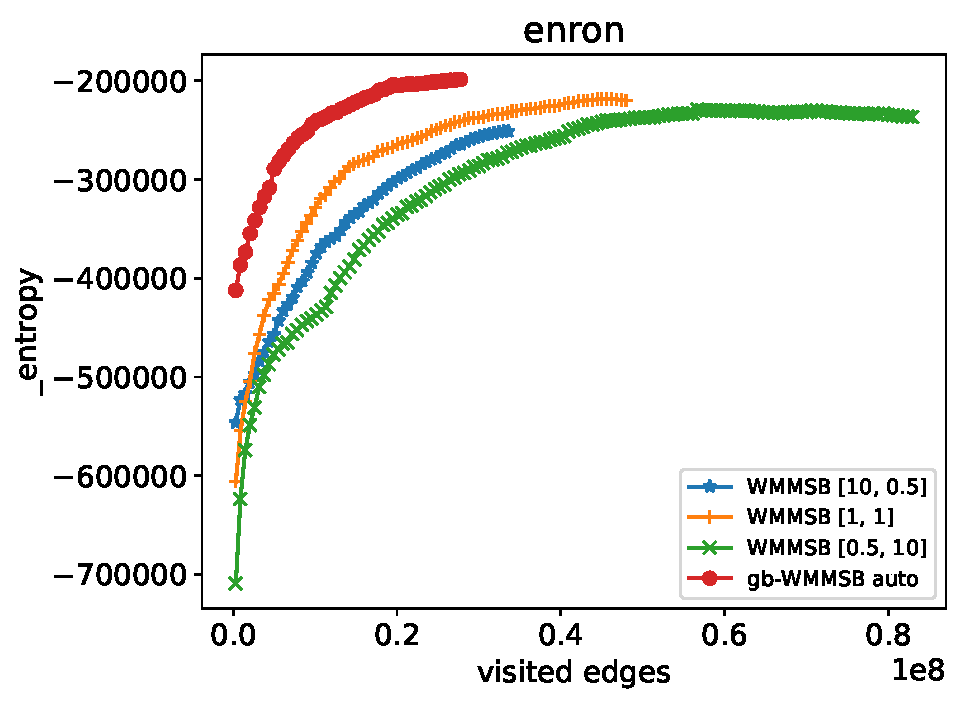
\includegraphics[width=0.32\textwidth]{warm2/enron_fig__entropy}
\end{subfigure}
\begin{subfigure}
         \centering
      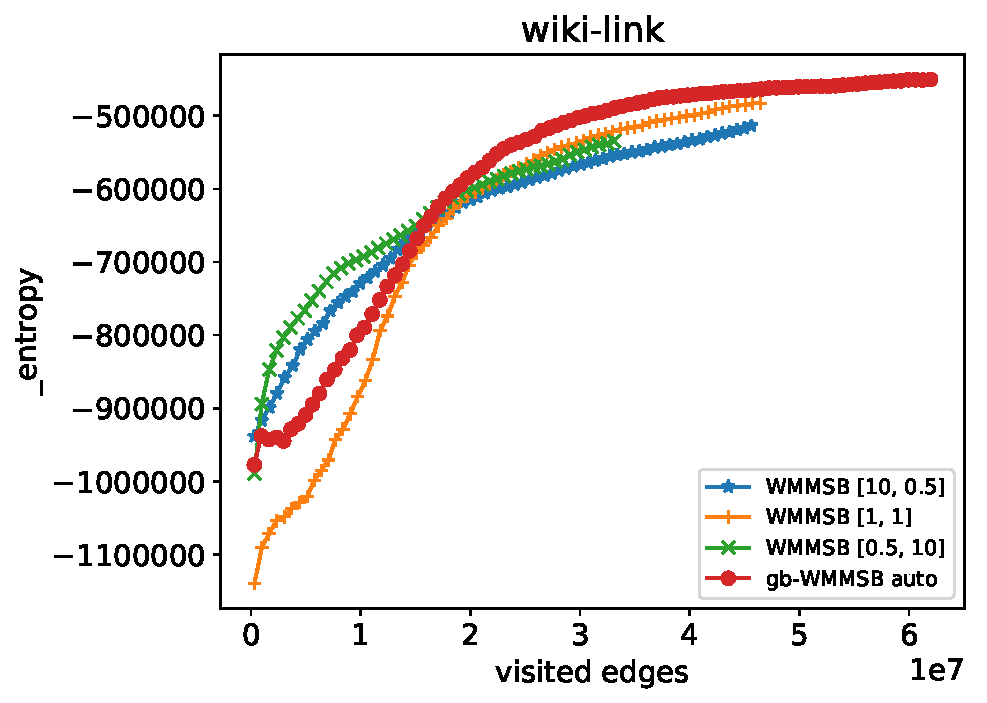
\includegraphics[width=0.32\textwidth]{warm2/wiki-link_fig__entropy}
\end{subfigure}
\begin{subfigure}
         \centering
      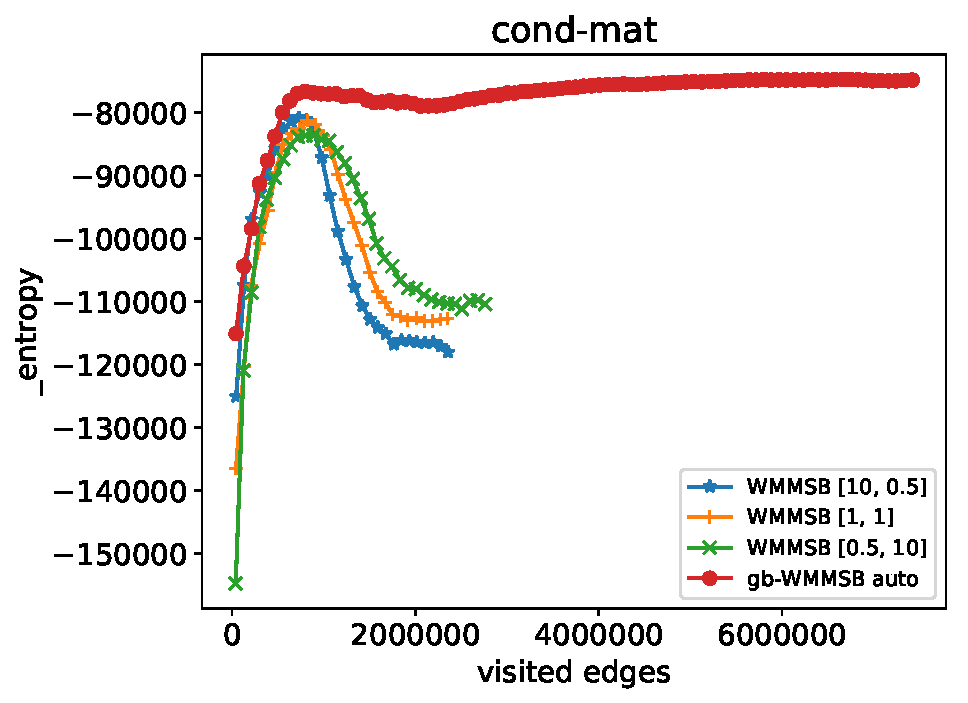
\includegraphics[width=0.32\textwidth]{warm2/cond-mat_fig__entropy}
\end{subfigure}
\caption{Log-likelihood convergence for WMMSB for different gamma prior. The bg-WMMSB model converges faster compared to fixed Gamma settings.}

%    \label{fig:conv_entropy}
%\end{figure}

%
% Sim
%
%For the weighted models, we further measure the capacity to predict right edge counts with a $l_1$ distance between the real count of the test set and the expected count of the models 
%
%\begin{equation*}
%D_{l_1}(D_{test} ||  \{\Thetah, \Phih\}) = \sum_{i,j \in \D_{test}} | y_{ij} - \E[y_{ij}|\Thetah, \Phih] |
%\end{equation*}






